%% ch6_V_a  第五章：紧合性的赋值判据，原书 pp. 34--36
\section{紧合性的赋值判据：全局与局部稳定化}

我们始终固定：
$X$ 为 $\mathbb{F}_{q}$ 上的射影、光滑、几何连通曲线，
$r=$ 秩，$d=$ 次数，$p:[0,r]\to\mathbb{R}_{+}$ 为凸截断多边形。

我们要证明
\[
\overline{\mathrm{Cht}^{r,d,\bar{p}\le p}}\qquad(\supset\mathrm{Cht}^{r,d,\bar{p}\le p})
\]
满足紧合性的赋值判据。

于是设：
$A=$ 离散赋值环，
$K_{A}=\mathrm{Frac}(A)$，
$\kappa_{A}=$ 剩余域，
$\pi_{A}=$ 一致化子。

考虑正则曲面\footnote{译注：原文以左侧一个大括号标出曲面 $X\otimes A$，以左下角一个小括号标出底概形 $\mathrm{Spec}A$；此处以连线代替括号。图中左侧细线为特殊纤维 $X\otimes\kappa_{A}$，右侧粗线为一般纤维 $X\otimes K_{A}$，横线为 $\mathrm{Spec}A_{X}$。[来源：转录稿图注 p.~35]} $X\otimes A$：
\origpage{35}
\begin{center}
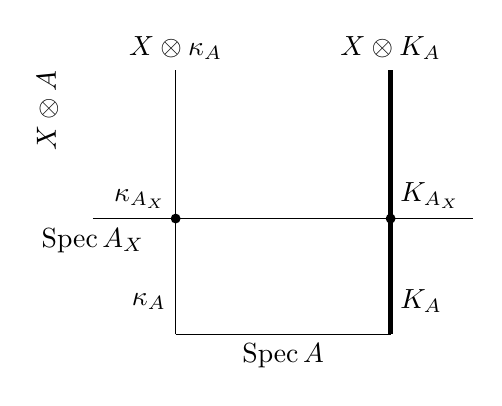
\begin{tikzpicture}[scale=1.05]
  \draw (0,0) -- (2.6,0);
  \node[below] at (1.3,0) {$\mathrm{Spec}\,A$};
  \draw[line width=0.5pt] (0,0) -- (0,3.2);
  \draw[line width=1.8pt] (2.6,0) -- (2.6,3.2);
  \node[above] at (0,3.2) {$X\otimes\kappa_{A}$};
  \node[above] at (2.6,3.2) {$X\otimes K_{A}$};
  \node[left] at (0,0.4) {$\kappa_{A}$};
  \node[right] at (2.6,0.4) {$K_{A}$};
  \draw (-1.0,1.4) -- (3.6,1.4);
  \node[below] at (-1.0,1.4) {$\mathrm{Spec}\,A_{X}$};
  \fill (0,1.4) circle (1.7pt);
  \fill (2.6,1.4) circle (1.7pt);
  \node[above left] at (0,1.4) {$\kappa_{A_{X}}$};
  \node[above right] at (2.6,1.4) {$K_{A_{X}}$};
  \node[rotate=90] at (-1.55,2.7) {$X\otimes A$};
\end{tikzpicture}
\end{center}

这里 $A_{X}$ 记 $X$ 在其特殊纤维 $X\otimes\kappa_{A}$ 的泛点处的局部环。它是离散赋值环；其剩余域 $\kappa_{A_{X}}$ 是 $X\otimes\kappa_{A}$ 的函数域，其分式域则是 $X$ 的函数域，也是其一般纤维 $X\otimes K_{A}$ 的函数域。

任取一个点
\[
\tilde{\mathcal{E}}\in\mathrm{Cht}^{r,d,\bar{p}\le p}(K_{A});
\]
我们要证明它在
\[
\overline{\mathrm{Cht}^{r,d,\bar{p}\le p}}(A)
\]
中有唯一延拓。

把
\[
\tilde{\mathcal{E}}=(\mathcal{E}\hookrightarrow\mathcal{E}'\hookleftarrow\mathcal{E}''\xleftarrow[\sim]{u}{}^{\tau}\mathcal{E})
\]
写成 $X\otimes K_{A}$ 上丛的图表。

设 $V$ 为 $\mathcal{E},\mathcal{E}',\mathcal{E}''$ 的一般纤维，即 $K_{A_{X}}$ 上一个维数 $r$ 的空间，带有
\[
{}^{\tau}V\xrightarrow[\sim]{u}V\qquad(V=\text{「}\varphi\text{-空间」}).
\]

\begin{lemma*}
$X\otimes A$（正则曲面）上丛的范畴，等价于一般曲线 $X\otimes K_{A}$ 上丛连同其一般纤维的一个格的范畴。
\end{lemma*}

$V$ 中每个 $A_{X}$-格 $M$ 都诱导出
\[
\mathcal{E}(M)\hookrightarrow\mathcal{E}'(M)\hookleftarrow\mathcal{E}''(M)\quad\text{即 }X\otimes A\text{ 上的丛}
\]
\origpage{36}其中的商自动支撑在
\[
\infty,0:\operatorname{Spec}A\rightrightarrows X
\]
的图像上。

限制之后得到
\[
\mathcal{E}^{M}\hookrightarrow\mathcal{E}'{}^{M}\hookleftarrow\mathcal{E}''{}^{M}\quad\text{即 }X\otimes\kappa_{A}\text{ 上的丛}
\]
其一般纤维为
\[
V^{M}=M/\pi_{A}M.
\]

它是 $A$ 上的 chtouca，当且仅当
\[
M=\text{「}\varphi\text{-格」}
\]
意思是
\[
{}^{\tau}V\xrightarrow[\sim]{u}V\quad\text{诱导出}\quad{}^{\tau}M\xrightarrow{\sim}M.
\]

\par\medskip\noindent\textbf{事实.}\ 唯一性没有问题（$\mathrm{Cht}^{r}$ 分离），但 $\varphi$-格未必存在。此外，即便存在 $\varphi$-格，它所诱导的 chtouca 也可能落在 $\mathrm{Cht}^{r,d,\bar{p}\le p}$ 之外。

\begin{definition*}
关于整数 $d_{1},\ldots,d_{r-1}\ge 0$ 的「迭代 $\varphi$-格」$M$，指的是 $V$ 的一个 $A_{X}$-格 $M$，使得若令
\[
u_{s}=\Big(\prod_{1\le t<s}\pi_{A}^{d_{t}(s-t)}\Big)^{-(q-1)}\Lambda^{s}u,\quad 1\le s\le r,
\]
则每个 $u_{s}$ 都诱导出一个良定义的态射
\[
u_{s}:{}^{\tau}\Lambda^{s}M\to\Lambda^{s}M
\]
它在 $\Lambda^{s}(M/\pi_{A}M)=\Lambda^{s}V^{M}$ 上的限制 $\overline{u}_{s}$ 满足
\[
\overline{u}_{s}\ne 0\quad\text{且}\quad{}^{\tau}\Lambda^{s}V^{M}=\mathrm{Ker}(\overline{u}_{s})\oplus{}^{\tau}\mathrm{Im}(\overline{u}_{s}).
\]
\end{definition*}

% ============================================================
%  \cite 使用清单
%  本段（原书 pp. 28--36，PDF 第 29--37 页）原文没有方括号文献引用，
%  因此未使用任何 \cite。全书约定为「姓氏小写 + 两位年份」，例如
%  \cite{lafforgue97}、\cite{lafforgue98}、\cite{lafforgue02}、
%  \cite{drinfeld74}。
%
%  待定术语（术语表未收，此处暂定，待全书统一）
%  - strate：分层（术语表只收「strate de bord / 边界分层」）
%  - DCN (diviseur à croisements normaux)：正规交叉除子；相对者作「相对 DCN」
%  - polygone convexe de troncature：凸截断多边形（术语表收「截断多边形」）
%  - assez convexe：足够凸
%  - saut de pente：斜率跳跃
%  - trait：trait（离散赋值环的谱），保留原文
%  - générisation / spécialisation：一般纤维 / 特殊化
%  - revêtement ramifié：分歧覆盖
%  - Fait：事实
%  - « bon » sous-objet：「好」子对象；type I / type II：类型 I / 类型 II
% ============================================================
